% =====================================================================
% paper/thesis_ch5/sections/online.tex
% §5.5 在线情形下的可学习性与信息瓶颈
% =====================================================================
% rev.1（2026-06-17）：§5.5 首版落地。组织遵循高水平实证 RL 论文的"机制判别"骨架：
%   §5.5.1 亚临界工况可行性（传感配置可学习性初筛，A0 sensor screen）；
%   §5.5.2 临界工况下部分可观测性差距的显现 + 竞争假设的提出；
%   §5.5.3 单变量消融判别（特权信息 vs 时序访问）+ 物理机制；
%   §5.5.4 时序闭合稳健性 + 评估集经验上界；
%   §5.5.5 对可部署策略设计的含义（中心命题挂钩 + 失效边界伏笔）；
%   §5.5.m 实施细节与可复现性。
%   数字回查：online_rl_line_summary.md §1.1（A0）+ arrival_v2_experiment_report.md
%   §7.6–§7.9（临界工况 gap / 特权 critic 消融 / history k 消融 / manifest 经验上界）。
%   口径裁定：A0 用历史效率导向奖励（efficiency_v2，§5.3 早期设定）、prototype 用到达
%   导向奖励（arrival_v2，§5.3 正式主奖励）；不引入 arrival_v1（章中未定义）。在线评估
%   30 回合/种子（§5.3 在线检查点评估口径）；种子只报数量不列编号（§5.3 §5.3.6）。
%   硬约束守：① 红线 3——空间探针 s1 写作"有效但非必需、不可部署、时序访问可替代"，
%   不写"传感器无用"；② 特权 critic 不闭合 gap 写作反向轴在线印证，不与离线 N2' 并列
%   下结论（在线 floor 10% 仅作 §5.8 伏笔，用散文前指、不 \ref 未落地节）；③ 不提
%   LayerNorm（在线标准 SAC 无关）；④ 机制句不写硬涡街周期（与 §5.3 ~38s 不冲突），
%   只按控制周期 0.5s 推出时序窗秒数 + 定性"覆盖脱涡周期相当比例"；⑤ 语体学术化——
%   不用 PASS/FAIL/catastrophic/gate/run 等报告腔，越界=OOB、评估集=manifest，机制作主语。
%   不写任何 LayerNorm / 离线结论 / 跨源 headline。本节无新增 cite（SAC haarnoja2018sac、
%   非对称 pinto2017asymmetric 均已在 §5.4 引入）。
% rev.2（2026-06-17）：独立对抗复审修订落地。① 统计口径：删 §5.5.4 与 k=8 总体口径
%   标准差 0.181（与 k=12 样本口径 0.038 不一致），表 tab:ch5_online_bottleneck 收为
%   三行受控单变量对照（不再混排 n=1/n=3），k=12 重复训练稳健性下放正文散文。② 种子
%   表述克制（用户指示）：正文不再逐一列举种子编号/种子数/per-seed 数值，跨重复训练
%   稳健性以聚合趋势表述，单次受控对照视为可信结论；种子细节保留 §5.5.m 复现子节。
%   ③ 过断言收回：评估集"固有上限"→"经验上界"，补小样本(rule-of-three)限定、删"与
%   随机种子无关"；k=8"完全追平"限定为受控对照、稳健性 \ref §5.5.4；§5.5.2 80pp 差距
%   去绝对化。④ 机制降为假说措辞（"明确的物理解释"→"可由如下机制解释"、"正是同一
%   物理量"→"很可能对应"）；补维度-容量混淆排除（s1 低维即达上界）。⑤ 语体：删"值得
%   注意的是"、序数枚举"第一组/第二组消融"散文化、去口语副词与破折号堆叠。
% =====================================================================
% rev.3（2026-06-18）：§5.5 两图落地 + 临界工况升级为多 seed 实测后的数字同步。
%   ⚠ PRELIMINARY：临界传感比较（s0/s1/s2 @ k=4）与 k 扫描 k=4 锚点取自云端新跑三 seed，
%   结果文件未取回本地核对；落字 = 用户口述 per-seed（s0 .10/.35/.17、s1 .90/.87/.94、
%   s2 .80/.71/.92）算的均值±样本std。取回日志后须复核：§5.5.2 临界 s0 0.10→约0.21
%   /gap 80→约70pp/补 s2≈0.81；§5.5.3 历史消融 0.100→0.900 改均值 0.21→0.76（最佳种子
%   追平、稳健追平须 k=12）；瓶颈表改 k=4/8/12+s1 四行成功率均值±std（删越界率列，多 seed
%   OOB 未取回）；§5.5.5 floor 10%→均值约0.2；§5.5.m 临界传感比较补「各取三随机种子」。
%   未动：亚临界表/数字、特权消融 0.220→0.066（2-seed 与图一致）、k=8 未稳/k=12 σ=0.038/
%   经验上界 27/30。两图脚本：figures/scripts/fig_ch5_online_{learnability,bottleneck}.py。
% rev.4（2026-06-18）：§5.5 第二轮高标准复审 + 重写（学习曲线落地 / 判别链展开 / 语域提级）。
%   按高水平实证 RL 论文标准补足证据呈现，六图重排（旧两面板 learnability 图 + k线/特权臂
%   bottleneck 图退役）：
%     §5.5.1 亚临界改用学习曲线 fig_ch5_online_curves_subcrit（n=3 真实 eval_log）；
%     §5.5.2 临界传感对比单面板柱状 fig_ch5_online_sensing_crit（⚠PRELIMINARY，3-seed 口述待云端核）；
%     §5.5.3 时序消融学习曲线 fig_ch5_online_curves_ksweep（k=4/8/12 真实 eval_log）+ 样本效率；
%            特权 critic 反向轴学习曲线 fig_ch5_online_priv_critic；
%     §5.5.4 单调剂量响应 fig_ch5_online_monotonic + manifest universal floor
%            fig_ch5_online_manifest_floor（per-episode final_eval 重建 ep 8/16/28 → 27/30）。
%   数据忠实度修订（一手核 eval_log.csv / final_eval.json）：
%     ① 成功率口径统一并显式声明（§5.5.m）——表/柱=终检 final_eval(30ep)、曲线=周期评估(30ep,
%        3点滑动平均)、peak=周期峰值；原 §5.5.3「最终成功率 0.220→0.066」实为 mean39（训练期均值）
%        误标为 final，已删该数，改用稳健量（峰值跨种子锁 0.267 vs 标准 SAC 0.37–0.53 + 曲线全程更低）。
%     ② 删特权 critic 不稳健的行为度量（safety −34%/progress +64%/return +26% 系 seed42 单 seed，
%        两 seed 池均值 progress/return 方向反转），§5.5.3 不再写「更安全/更积极」。
%     ③ k=4 锚点改用本地 final_eval（n=2，≈0.25）与图一致；云端 3-seed（≈0.21，PRELIMINARY）取回后复核；
%        临界传感 s1/s2 仍 PRELIMINARY。
%   语域提级（§0.5.9 + 用户指示「正式论文不强调种子数/个别种子」）：删 speech-act 预告
%   （「是下一子节的考察对象」）、空元话语（「值得对照的是」「更值得重视的是其趋势」「初步提示」）；
%   方法学（种子数/数据来源）只在 §5.5.m 交代一次。保留真严谨：rule-of-three「经验上界非不可达
%   证明」、多 seed 稳健性必要性（语气由辩解改陈述）。红线沿守：红线3 s1=参照上界不可部署/时序可
%   替代；特权=反向轴在线印证不跨线；不提 LayerNorm；机制按 Δt 推时序窗不写硬涡街周期；在线 floor
%   作 §5.8 散文伏笔不 \ref。两图脚本族见 figures/scripts/fig_ch5_online_*.py + 共享 _ch5_data.py。
% rev.5（2026-06-18）：rev.3/rev.4 的 ⚠ PRELIMINARY 全部解除。临界传感比较 s0/s1/s2 @ k=4
%   云端三种子（seed 0/7/42, final_eval）已确认，并与本地 final_eval 交叉核对一致（s0 seed_0=.4
%   /seed_42=.1、s1 seed_42=.9）：s0=[.4/.267/.1]→0.26±0.15、s1=[.9/.8/.9]→0.87±0.06、
%   s2=[.8/.733/.733]→0.76±0.04，gap s1−s0=0.61（约60pp）。落地：① Fig sensing_crit 脚本
%   CRIT_SEEDS 改实测、去 PRELIMINARY、重绘；② §5.5.2 正文 s0 0.21→0.26 / s1 0.90→0.87 /
%   s2 0.81→0.76 / gap 70→60pp，caption 删 PRELIMINARY 句；③ 瓶颈表 k=4 行 0.25±0.21→0.26±0.15
%   （n=2→3，补 seed_7=.267）、s1 行 0.90→0.87±0.06（n=1→3）；④ §5.5.5 floor 约0.2→约0.26；
%   ⑤ 删 §5.5.m 双测量段（云端0.21 vs 本地0.25 二分作废——云端三种子即唯一权威读数、含本地两 seed），
%   k=4 种子数 2→3。数据忠实度新修正：真实 s2 离散度（std 0.04）< s1（std 0.06），删 §5.5.2/caption
%   「s2 离散度高于 s1」错述，改「s2 居中仍低于 s1」（信息更富未必更优，与亚临界一致）；Fig curves_ksweep
%   caption 删「0.90 与 s1 重合」（经验上界 0.90 系 manifest floor 27/30，独立于 s1=0.87）。未动：
%   特权消融 2-seed（用户未供云端 asym 数据）、k=8/k=12 本地三种子、经验上界 27/30。注：Fig curves_ksweep
%   的 k=4 学习曲线仍为 2-seed 周期评估（seed_7 周期 eval_log 未取回，仅 final_eval 标量已得），
%   与瓶颈表 k=4（3-seed 终检）口径不同已在 §5.5.m 声明，不构成矛盾。
% rev.6（2026-06-18）：系统性复审定点加固（保留 5 子节发现链骨架，不推翻数据）。
%   [H1 章级实施细节归属] §5.5.m ¶3 越界承载的"三种读数全章统一"段瘦身——"终检/周期评估"
%     命名上提到 §5.3.6（评估协议，全章唯一定义之家），§5.5.m 改为指针引用 + 只就近定义在线
%     特有的"峰值"读数；删与 §5.3 重复的种子编号约定。配套 setup.tex rev.4 / td3bc.tex rev.3。
%   [H2 图文/稳健性一致] §5.5.3 样本效率原以 k=8 单种子峰值"475k 步"立论，与图（k=12 seed-mean
%     峰值最早）+ §5.5.4（k=8 跨种子不稳）三处打架；改以 k=12 立论（渐近最高 + 峰值最早 + 达空间
%     参照水平快于 s1 自身约 72.5 万步），与图、与稳健性结论一致。
%   [H3 发现链] §5.5.2 三竞争假设，原 §5.5.3 只显式消融价值/时序两条；补开头映射句 + 机制段末
%     三假设各自收口（价值=反向消融排除、时序=正向消融锁定、空间信息=时序可替代故"有效但非必需"）。
%   [M 系列语体/数字] 单位"475/725 k 步"→"万步"（全章一致）；"全章预设的稳健阈值"去 gate 腔；
%     章引言"奠定基调"→"判断主线"；§5.5.1/§5.5.m"筛查"→"考察"；特权 critic 图-注-文统一到 0.267
%     （图脚本标注 0.27→0.267 重绘）。红线沿守（s1/s2 参照上界·时序可替代、特权=反向轴不跨线、
%     不提 LayerNorm、机制按 Δt 不写硬涡街周期、在线低水平作 §5.8 散文伏笔不 \ref）。
% 收尾统稿轮（2026-07-08）："沿船体"→"沿机体"×2（章级术语统一，用户裁定）；
%   fig priv_critic 与 fig curves_ksweep 两环境互换（首引序 146<148 与编号序对齐，
%   包 C 编号一致性）；tab bottleneck [t]→[htbp]。零数字/零论证改动。
% rev.7（2026-07-19）：临界传感九宫格重排（用户裁决：2026-06-18 转录值确认为引用
%   错误、完全作废（占位数字），以 2026-07-08 同协议补跑值为唯一 ground truth；
%   方案与裁决 = supplement plan 附录 B.1/C；数字权威 = arrival_v2_experiment_report.md
%   §7.10（✅ 9/9 本机实核，本轮已重写））。新值：s0=[.40/.867/.10]→0.46±0.39、
%   s1=[.90/.90/.90]→0.90±0.00、s2=[.867/.833/.90]→0.87±0.03，gap 0.61→0.44。
%   落地：① §5.5.2 正文——「几近失败 0.26」→「剧烈分化（0.10–0.87）、均值约 0.46」、
%   s1 0.87→0.90、「s2 居中仍低于 s1」→「与 s1 几乎并列」、gap 60→44pp；② caption 同步；
%   ③ §5.5.3 剂量响应句补跨种子方差单调收缩（std 0.39→0.22→0.04）新证据；
%   ④ 瓶颈表 k=4 行 0.46±0.39、s1 行 0.90±0.00（k=8/k=12 行经重算不变）；
%   ⑤ §5.5.4 ksweep caption 删「近底板」；⑥ §5.5.5 参照句「几近失败」→「无法被
%   可靠学得」、k=12 救援改述为「稳定抬升」（不可靠→稳定）。两图脚本 CRIT_SEEDS/
%   CRIT_K4_S0 改新值并重绘。核心结论（瓶颈在时序利用）不变；红线沿守（s1/s2 参照
%   上界不可部署、时序可替代，不引申「空间参照无用」）。§5.5.m 无改动。
% =====================================================================

% 第 3 批整改（2026-07-22，重流程；findings §8 N1 同类收口）：§5.5.2 特权 critic
%   消融段「表明它反映**该信息配置所能达到的上限**，而非随机波动」——该消融只有两
%   随机种子（§5.5.m），以 n=2 的峰值一致性断言「所能达到的上限」属 N1 同一错误
%   类别（把某配置下的读数讲成上限），且 §5.10.3 本批新增句把在线一侧提到收束层、
%   暴露面加大 → 改「表明它反映的是**该信息配置下重复训练间稳定复现的水平**，而非
%   随机波动」。§5.5.4「时序访问所能达到的上限」指评估集自身上界、正文已带
%   「观测到的经验上界而非严格的不可达性证明」+ 五次训练基底，属合法用法，不动。
%   零数字/零论证改动。
%
% rev.8（2026-07-24）：全章复审整改第 4 批（重流程；findings H4 / H7 / M1）。本节三处：
%   [H4·§5.5.3] 机制段后**另起一段**（3 句）补文献坐标与增量定位：帧堆叠携带时序信息
%     是缓解部分可观测性的通行做法（mnih2015dqn）、从局部流速时序刻画流动结构已有先例
%     （colvert2018wakes）；本章增量精确定位为「把时序窗所恢复的信息**指认为涡街脱落
%     的相位**，并以受控消融证明该恢复**足以替代空间多点探针**」，而非「观测历史有用」。
%     ⚠ 另起一段而非并入机制段：机制段本已 7 句以上，插句会加剧 findings §9 N11 的
%     段长偏离；新段 3 句守 §0.5.7。
%   [H7·§5.5.4] 「决定性的证据在其单调性…这一攀升在**单次训练内部**即沿 k=4→8→12
%     重现」经 GT 实核为**选择性呈现**——图中「单次代表性训练」取的是三种子中唯一严格
%     单调者（seed 0：0.40→0.50→0.90），而 seed 7 实为 0.867→0.867→**0.833**（持平后
%     微降），且 k=4 最好种子（0.867）**高于** k=12 最差种子（0.833）。本机 9/9 实读
%     final_eval.json 确认（k=4 [0.40/0.867/0.10]、k=8 [0.50/0.867/0.90]、
%     k=12 [0.90/0.833/0.90]），与 arrival_v2_experiment_report.md §7.9/§7.10 逐格一致。
%     → 改述为「三次训练中两次单调、一次在高位持平后微降」，**论点重心移到方差收缩**
%     （σ 0.39→0.22→0.04，§5.5.3 已刊）。
%     ⚠ 「排除两种竞争解释」是否受损——正面结论：**不受损，反更干净**。方差收缩本身
%     即「坏种子被一致清除」的直接度量，比单条轨迹的单调性更贴合「排除初始化局部极小」；
%     GT §7.9.2 F2.3 亦明言 seed 0 的跨历史救援（k=8 0.50 → k=12 0.90，同 init）是
%     information-capacity 而非 init-basin。原论证挂在单调性上，会被 seed 7 一击；移到
%     方差收缩后无此软肋。图 caption 与绘图脚本同步（脚本改画三条逐种子轨迹，不再前置
%     单条最强种子）。
%   [M1·§5.5.3] 特权 critic 段补口径限定（新增段，3 句）：正文结论取**周期评估**口径
%     （曲线与峰值）；**终检**口径下两者终点成功率相差仅数个百分点且**方向相反**
%     （GT §7.7：特权 0.167 vs 标准 0.100，GT 明言该 +6.7pp 系 30 回合评估上 2 个回合
%     之差、属噪声），故就地声明两种口径下「差距未被缩小」的判断均成立、不依赖口径。
%     ⚠ 不写终检两个数字字面量（避免向 §5.5.3 引入两个章内未有的读数）。
%     ⚠ 与第 3 批新文本的交互已核：discussion.tex §5.10.3 正文与表 5.21 第 1 行均用
%     「**收敛峰值**」（周期评估口径），与本口径限定一致，**无需同步改**。
%   ⚠ **上述三处的初稿均经四维度独立对抗复审推翻，本 rev 为重做后定稿**（合并去重
%     CRIT 4 / HIGH ~11，远超 §5.9 基线 4，触发退回）。三处推翻理由如实记录：
%     ① **H7 的替代论证比它替换掉的更弱**（复审 B）：初稿把判别力从「单次训练内部
%        单调」移到「跨重复训练的离散度收缩」，但 σ 收缩 (a) 只度量**症状被清除**、
%        不识别**病因**——任何使优化更容易的干预都会治好 init-basin 型弱训练；
%        (b) 受**天花板混杂**——k=12 三读数 {0.90, 0.833, 0.90} 有两个恰压在紧邻
%        下一段才建立的经验上界 0.90 上，均值逼近硬上界时 σ 必然收缩，故它是均值
%        抬升的**导出量**而非独立证据，相邻两段自相拆台；(c) 末端**低于评估噪声地板**
%        ——30 回合、p=0.9 的二项抽样标准差 $\sqrt{0.9\cdot0.1/30}=0.055$ 已大于所报
%        σ=0.04；(d) **GT 从不用 σ 作判别器**——`arrival_v2_experiment_report.md`
%        §7.9.2 F2.3 / §7.9.3 把 H_seed-stall 与 H_optimization-noise 的证伪完全挂在
%        **同一 init seed 下的跨 k 救援**（seed 0：k=8 的 0.500 → k=12 的 0.900）上，
%        σ 在 GT 里只是 thesis-grade 稳健性指标。→ 定稿改挂**同一初始化下的跨历史
%        长度对照**（GT 的原论证），σ 退为「与这一图景一致、但末端受上界与评估规模
%        所限，只作稳健性旁证」。段回 4 句。
%     ② **H4 段「精确指认／证明」与紧邻上一段的假说措辞直接冲突**（复审 A/B/C 三维
%        同时命中）：机制段（本节上一段）三重对冲「**可能**从时序节拍中反演」「**很可能**
%        对应」「**若如此**」，下一段即宣称「**精确指认**为涡街脱落的相位」「**证明**这一
%        恢复足以替代」——先撤销许可再照旧行使，正是第 3 批栽掉的形态。相位从未被
%        直接测量（GT §7.9.3 同样只以时间尺度吻合支持该假说）；且「以受控消融**证明
%        这一恢复**足以替代」把主语从「延长时序窗」偷换为「相位恢复」，把未证机制
%        夹带进已证的替代命题。→ 定稿降为「**指向**涡街脱落的相位这一具体的物理
%        候选」＋「**表明**……足以在**任务级上**替代」，并补 scope（在线临界工况与所
%        考察的时序窗范围）。另删「本章在此之上的增量，**不在于**重申观测历史有用，
%        **而在于**……」——复审 D 判其双犯 §0.5.9(a)（宣告 novelty ＋ 反向宣告），
%        且「增量」是 rev 头注的工程语域渗入正文；定位红线改由前句的文献坐标自证。
%     ③ **M1「方向相反」系单种子挑选**（复审 A/B 双命中，本机 `final_eval.json` 实读
%        复核）：本节口径是**两种子配对复现**，而 seed 42 为 0.100 vs 0.167（特权高）、
%        seed 0 为 0.400 vs 0.200（特权低），**配对均值 0.250 vs 0.184、特权仍低约
%        6.6pp，方向并未相反**。初稿取了三个可用读数中唯一支持「方向相反」的那个，
%        与本批 H7 所要根除的病因同型。→ 定稿如实写「配对复现两次训练的**均值**仍以
%        接收特权观测的价值网络为低、与周期评估口径**同向**；两次训练各自的方向并不
%        一致」。诚实版本反而更强。**新增「三十回合评估上两个回合」一个计数**（GT §7.7
%        原口径「30-ep eval 上 2 个 episode 的差」），以替换初稿无量的「落在抽样噪声
%        之内」；属 GT 搬运、非成功率读数。
%     ④ 结构与措辞连带（复审 D）：M1 口径段初稿被楔入「证据 → 结论」之间，制造单句
%        孤段并倒置 §0.5.7 的「finding → interpretation → caveat」序 → 结论句并回原段，
%        口径段整体下移作独立 caveat；「观测帧堆叠」→「**历史堆叠**」（定义之家 §5.3.2
%        既有形，原为全章孤例）；「特权价值网络」→「**特权协议**」（§0.5.10 (B) 档）；
%        图 caption 去「剂量响应」（全章孤例，且该药理隐喻恰指单调分级、与 H7 的后撤
%        自相矛盾）。
%     ⑤ **措辞锁失守收口**（复审 C）：§5.5.4 行首「单次受控对照上的**追平**」——第 3 批
%        H2 明令禁用词，而本批**逐字改写了该行后半句却未触碰行首**；§5.5.3 两处
%        「与空间参照水平**相当**」「恢复到与空间参照**一致的水平**」同属该锁，且正是
%        新增量断言的承重件（上游是无兜底的等价判断，下游被升格为「足以替代」）。
%        三处已改为「检测不出差距／未见可检出的差距／回升到……水平附近」。
%   零新数字字面量（H7 以定性表述承载；M1 仅增一个 GT 计数，见 ③）；本批新增文本
%   零破折号（findings §9 N10；复审 D 实算确认全章正文段密度 0.615 → 0.593，反向改善）。
\section{在线情形下的可学习性与信息瓶颈}\label{sec:ch5_online}

\S\ref{sec:ch5_intro} 把在线情形定位为离线结果的解释基准：它考察任务在仅有单点局部感知时能否经由在线交互学会，以及性能受何种因素制约。本节以在线最大熵方法 SAC（\S\ref{subsec:ch5_method_sac}）在 \S\ref{subsec:ch5_task} 给定的两个流动工况上回答这一问题。在亚临界主工况，可部署的单点传感配置已具备基础可学习性；转入临界工况后，可部署配置与更丰富空间感知之间出现显著的性能差距，一组单变量消融将这一差距归因于策略对单点观测的时序利用，而非传感硬件或价值估计的不足。这一归因给出了全章中心命题的第一个落点：在固定的部署传感接口下，可部署性能的瓶颈主要落在如何利用既有观测，而不在于是否为系统增添新的感知能力；这一判断将在离线情形与失效边界的考察中反复得到印证与界定。

\subsection{亚临界工况下的可学习性与传感配置}\label{subsec:ch5_online_feasibility}

作为后续比较的前提，先在亚临界主工况下考察三种传感配置的基础可学习性。任务为 \S\ref{subsec:ch5_task} 所述的横流穿越，流动取来流 $U_\infty=1.0$ m/s、雷诺数 $\mathrm{Re}=150$；可部署的单点配置 $s_0$ 与两种空间参照配置 $s_1$、$s_2$（\S\ref{subsec:ch5_obs_deployable}，表~\ref{tab:ch5_sensor_family}）在历史效率导向奖励下以 $k=4$ 历史堆叠送入标准 SAC 训练，并在固定评估集上以确定性策略评估。表~\ref{tab:ch5_a0_sensor} 给出三种配置的任务成功率与成功回合的路径效率，图~\ref{fig:ch5_online_curves_subcrit} 给出对应的训练过程。

三种传感配置在这一工况下都达到可观的成功率，最弱者亦不低于 $0.78$，表明在亚临界尾流中任务对各传感配置均可学，无须先验地排除任何一种。可部署的单点配置 $s_0$ 成功率为 $0.789$，与最优的 $s_1$ 之间仍有差距，但其绝对水平已足以支撑可靠的横流穿越，路径效率（$0.801$）亦与 $s_1$（$0.854$）相近，说明在简单工况中仅凭单点流速即可学得高质量的运动规划。信息最丰富的 $s_2$ 却并未取得最高且最稳的表现：其成功率（$0.856$）低于 $s_1$，训练过程的离散度也明显更大，整段训练中其成功率带始终宽于 $s_1$（图~\ref{fig:ch5_online_curves_subcrit}）。更多的观测通道在此并未转化为更稳定的训练，反因输入维度升高而抬高了收敛难度——传感信息的丰富程度与可部署性能之间并非单调对应。

上述结果取自亚临界主工况的横流穿越任务，其结论限于这一相对易学的设定。一旦工况推进到临界区间，标准 SAC 在相同训练预算内已不能从单点观测稳定学得有效策略，可部署单点感知与更丰富空间感知之间的差距随之显现。

\begin{table}[t]
\centering
\caption{亚临界主工况（$\mathrm{Re}=150$、$U_\infty=1.0$ m/s）横流穿越任务下三种传感配置的在线可学习性。采用历史效率导向奖励、$k=4$ 历史堆叠，报告重复训练的均值 $\pm$ 标准差；成功率为终检评估下质心进入目标半径内的回合占比，路径效率为成功回合的航程效率（越接近 $1$ 表示路径越省）。粗体为各列最优。随机种子数与评估口径见 \S\ref{subsec:ch5_online_impl}。}
\label{tab:ch5_a0_sensor}
\begin{tabular}{lcc}
\toprule
\textbf{传感配置} & \textbf{成功率} & \textbf{路径效率} \\
\midrule
$s_0$（可部署，单点 DVL） & $0.789 \pm 0.211$ & $0.801 \pm 0.057$ \\
$s_1$（$+$ 短程 ADCP，参照上界） & $\mathbf{0.967 \pm 0.027}$ & $\mathbf{0.854 \pm 0.024}$ \\
$s_2$（$+$ 长程 ADCP，参照上界） & $0.856 \pm 0.204$ & $0.813 \pm 0.100$ \\
\bottomrule
\end{tabular}
\end{table}

\begin{figure}[htbp]
    \centering
    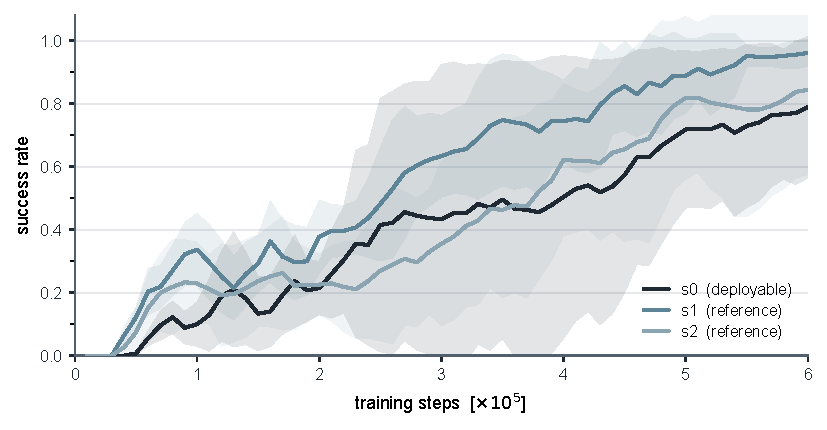
\includegraphics[width=138mm]{figures/fig_ch5_online_curves_subcrit.pdf}
    \caption{亚临界主工况（$\mathrm{Re}=150$、$U_\infty=1.0$ m/s，历史效率导向奖励）下三种传感配置的在线学习曲线，以标准 SAC 训练、确定性策略评估所得任务成功率（均值与种子带，曲线经轻度滑动平均）。三种配置均可学；信息最丰富的 $s_2$ 训练过程的离散度全程大于 $s_1$，更多观测通道未换来更稳的训练。$s_1$、$s_2$ 为参照上界，在部署中不可得。}
    \label{fig:ch5_online_curves_subcrit}
\end{figure}

\subsection{临界工况下部分可观测性差距的显现}\label{subsec:ch5_online_gap}

将工况推进到临界区间，可部署单点感知的局限才充分暴露。自本节起，分析改用本章正式的到达导向奖励，流动取 $U_\infty=1.5$ m/s、$\mathrm{Re}=250$，涡旋更强、脱落更快，速度比 $\lambda=1.0$ 使航行器形成稳定对地位移的速度余量大幅收缩。在此工况下，仅用单点观测且仅作 $k=4$ 历史堆叠的可部署配置已不能稳定完成横流穿越任务：重复训练的成功率在 $0.10$ 至 $0.87$ 之间剧烈分化，均值仅约 $0.46$，失败回合多因越出流场边界所致。同一任务下，仅增设一处前向探针的空间参照配置 $s_1$ 即在各次重复训练中一致达到约 $0.90$ 的成功率，信息更丰富的 $s_2$（约 $0.87$）与之几乎并列而未见额外增益，与亚临界工况一致地表明更多通道未必换来更好的可学习性。可部署配置与空间参照之间由此张开约 $44$ 个百分点的平均成功率差距，且前者深受初始化随机性摆布、后者高度一致，标示出临界工况下单点局部可观测所付出的代价（图~\ref{fig:ch5_online_sensing_crit}）。

\begin{figure}[htbp]
    \centering
    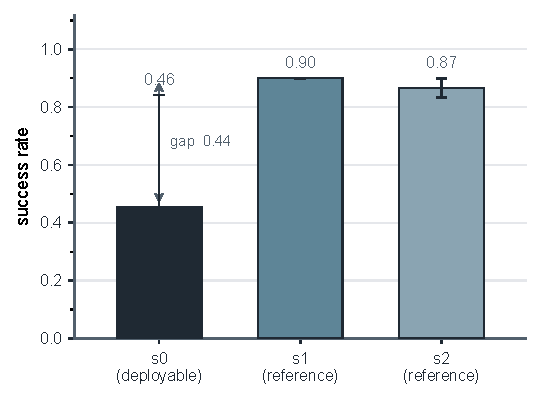
\includegraphics[width=90mm]{figures/fig_ch5_online_sensing_crit.pdf}
    \caption{临界工况（$\mathrm{Re}=250$、$U_\infty=1.5$ m/s，到达导向奖励）下三种传感配置的任务成功率（均值 $\pm$ 标准差）。可部署单点 $s_0$ 在重复训练间剧烈分化、均值仅约 $0.46$，仅增设一处前向探针的 $s_1$ 即一致守住约 $0.90$，信息更丰富的 $s_2$ 与 $s_1$ 几乎并列；可部署配置与空间参照之间张开约 $44$ 个百分点。$s_1$、$s_2$ 为参照上界，在部署中不可得。}
    \label{fig:ch5_online_sensing_crit}
\end{figure}

这一差距可能源于若干不同性质的瓶颈。一种可能是单点观测本身携带的空间信息不足，须以更多探针在空间上补足；另一种是价值网络对动作价值的估计不够准确，使策略改进的方向失真；还有一种是策略网络未能充分利用单点观测随时间的变化，因而损失了本可从时序中恢复的流场信息。这三者指向截然不同的干预——增设空间探针、改善价值估计、延长观测时序——对部署可行性也意味着不同的判断。它们是部署接口下可供干预的几条主要途径；下面以一组单变量消融逐一甄别，每次只改变基线配置中的一个因素、冻结其余训练条件，从而将成功率的变化明确归因于该因素。

\subsection{瓶颈的判别：特权信息与时序访问的单变量消融}\label{subsec:ch5_online_ablation}

前述三种可能里，价值估计与时序利用可经单变量消融直接检验，而单点空间信息是否不可替代，则由这两项消融的结果共同回答。判别从价值一侧入手，检验差距是否源于价值估计的不足。沿用 \S\ref{subsec:ch5_method_protocol} 给出的特权协议，在策略网络只读单点观测、唯一改变价值网络可见信息的前提下，向价值网络注入沿机体的等效来流估计这一特权观测~\citep{pinto2017asymmetric}。配对复现表明，这一改动并未缩小差距：可部署成功率在整个训练过程中始终低于标准 SAC，其收敛峰值跨重复训练稳定锁定在约 $0.267$，明显低于标准 SAC 的峰值区间（约 $0.37$–$0.53$）与空间参照配置（图~\ref{fig:ch5_online_priv_critic}）。峰值跨种子的这一稳定锁定，表明它反映的是该信息配置下重复训练间稳定复现的水平，而非随机波动。可见差距并不出在价值网络的估计精度：把训练期才有的特权信息提供给价值网络，并不能经由仅有单点观测的策略兑现为任务级的成功——瓶颈落在策略一侧可获取的信息，而非价值一侧的估计能力。

上述比较取周期评估口径，即整条学习曲线及其峰值。改用终检口径时（\S\ref{subsec:ch5_online_impl}），配对复现两次训练的均值仍以接收特权观测的价值网络为低，与周期评估口径同向；两次训练各自的差异方向并不一致，其中一次的差距仅合三十回合评估上两个回合，落在该评估规模的抽样噪声之内。两种口径下特权协议都远未把成功率抬近空间参照的水平，差距未被实质缩小这一判断因而不依赖于所取口径。

另一组消融转而作用于策略一侧的信息。在同一可部署基线上，唯一改变的是策略网络的观测历史长度，由 $k=4$ 依次增至 $k=8$、$k=12$，即把送入策略的时序窗由约 $2$ s 扩展到约 $4$ s 与约 $6$ s（控制周期 $\Delta t_{\mathrm{ctrl}}=0.5$ s）。在这一受控对照下，可部署配置的成功率随时序窗延长而系统性回升，失败回合的越界亦大幅减少：均值由约 $0.46$ 升至 $k=8$ 的约 $0.76$、再至 $k=12$ 的约 $0.88$，与空间参照之间未见可检出的差距，并贴近评估集的经验上界；更为显著的是重复训练间的离散度随时序窗延长单调收缩（标准差 $0.39\to0.22\to0.04$），时序窗延长不仅抬高了平均性能，更把 $k=4$ 下对初始化的剧烈敏感性压成一致收敛（图~\ref{fig:ch5_online_curves_ksweep}、表~\ref{tab:ch5_online_bottleneck}）。时序窗延长不仅抬高了渐近性能，也改善了样本效率：在三种历史长度中 $k=12$ 渐近水平最高，其收敛峰值也最早到达（图~\ref{fig:ch5_online_curves_ksweep} 中圆点）；可部署单点配置在 $k=12$ 下达到空间参照水平所需的训练步数，甚至少于空间参照配置自身（后者的收敛峰值约在 $72.5$ 万步）。与此相对，低维的空间参照配置 $s_1$ 以更短的历史即可达到同等水平，可见高成功率并不依赖更高的输入维度，时序窗延长带来的增益不能归于输入规模的扩大。两组消融形成鲜明对照：把等效来流信息提供给价值网络，任务级成功率不升反降；把同等数量级的时序信息提供给策略网络，成功率则随时序窗延长回升到空间参照的水平附近。

这一对照可由如下物理机制解释。临界工况下驱动航行器的主导扰动是周期性的涡街脱落；单点探针虽只测得当前位置的瞬时流速，但其随时间的变化编码了这一周期性脉动的相位。当策略只能看到单帧观测时，它无法区分同一流速值处于脉动的上升相还是下降相；而当时序窗覆盖脱涡周期的相当比例时，策略便可能从单点流速的时序节拍中反演出主导脉动的相位，进而预判流场的演变。这一相位信息很可能对应于价值网络在特权协议下通过沿机体等效来流所获取的同一脉动量。若如此，则可部署的单点传感并不缺少这一信息，只是它分布在时间维度而非空间维度上；空间上多设探针与时间上延长历史，便是获取同一相位信息的两条途径，而后者无须任何部署阶段不可得的传感。至此，临界差距所引出的三种可能各有归宿：价值估计的不足由反向消融排除，时序利用的不足由正向消融锁定为差距的主因，而单点空间信息不足这一可能，则因时序访问足以替代空间相位信息而被界定为有效但非必需——增设空间探针确能闭合差距，却非闭合差距的唯一或必要途径。

以历史堆叠把时序信息带入策略输入，是缓解部分可观测性的通行做法~\citep{mnih2015dqn}；从单点测量的时序变化刻画流动结构亦有先例，只是所测为涡量，而非本章可部署传感所能提供的流速~\citep{colvert2018wakes}。本节据此把时序窗所恢复的信息指向涡街脱落的相位这一具体的物理候选，并以上述受控消融表明，在这一在线临界工况与所考察的时序窗范围内，该恢复足以在任务级上替代空间上的多点探针。

\begin{figure}[htbp]
    \centering
    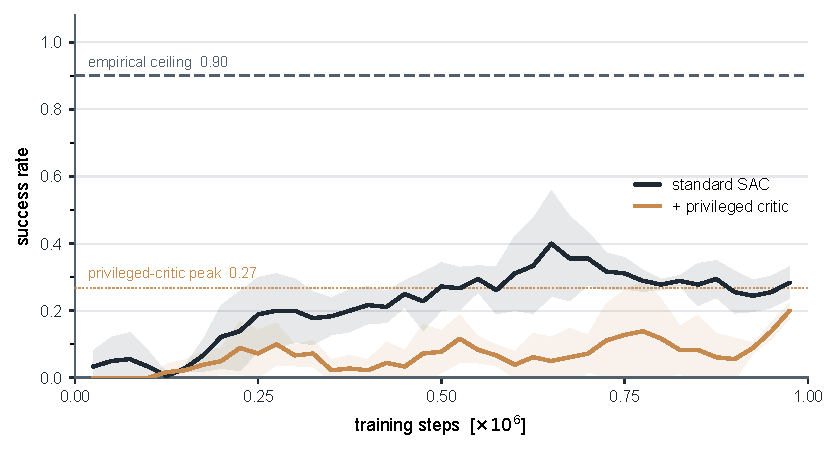
\includegraphics[width=138mm]{figures/fig_ch5_online_priv_critic.pdf}
    \caption{反向对照：临界工况下向价值网络注入特权来流观测对可部署成功率的作用（学习曲线，均值与种子带，曲线经轻度滑动平均）。自同一 $k=4$ 基线，注入特权观测后成功率在整个训练过程中低于标准 SAC，其峰值跨重复训练稳定锁定在约 $0.267$（暖色点线）而不能逾越——与延长时序窗的方向相反。可部署性能的瓶颈在策略对单点观测的时序利用，而非价值一侧的信息或估计能力。}
    \label{fig:ch5_online_priv_critic}
\end{figure}

\begin{figure}[htbp]
    \centering
    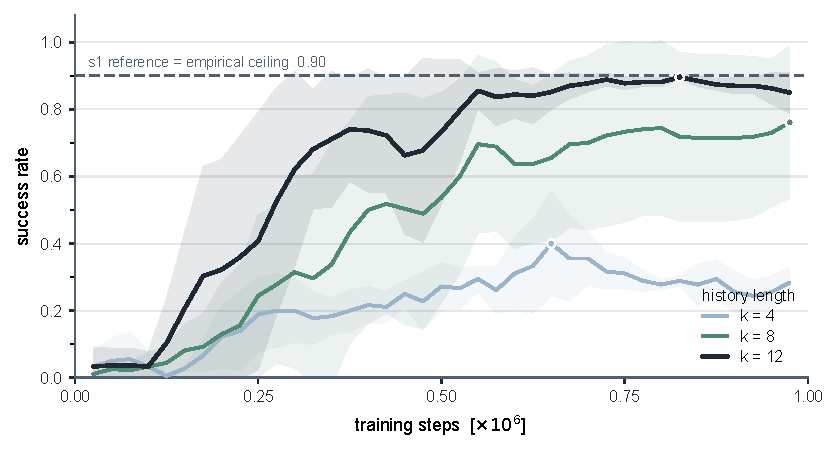
\includegraphics[width=138mm]{figures/fig_ch5_online_curves_ksweep.pdf}
    \caption{临界工况（$\mathrm{Re}=250$、$U_\infty=1.5$ m/s，到达导向奖励）下可部署单点 $s_0$ 的在线学习曲线随观测历史长度 $k$ 的变化（均值与种子带，曲线经轻度滑动平均；上轴为对应时序窗 $k\cdot\Delta t_{\mathrm{ctrl}}$，$\Delta t_{\mathrm{ctrl}}=0.5$ s）。随时序窗延长（$k=4\to8\to12$），成功率逐级抬升，并向评估集经验上界（$0.90$，灰色虚线）收敛；$k=12$ 不仅渐近水平最高，且达到峰值最早（圆点），即时序访问同时改善了渐近性能与样本效率。}
    \label{fig:ch5_online_curves_ksweep}
\end{figure}

\begin{table}[htbp]
\centering
\caption{临界工况（$\mathrm{Re}=250$、$U_\infty=1.5$ m/s）横流穿越任务下时序访问对可部署成功率的作用，采用到达导向奖励。各行只改变所标变量、冻结其余训练条件；成功率为终检（final-checkpoint）评估，报告重复训练的均值 $\pm$ 标准差。可部署单点 $s_0$ 的成功率随历史长度 $k$ 上升，并向空间参照 $s_1$（$k=4$）与评估集经验上界（$27/30=0.90$）收敛。各行随机种子数与数据来源见 \S\ref{subsec:ch5_online_impl}。}
\label{tab:ch5_online_bottleneck}
\begin{tabular}{lc}
\toprule
\textbf{配置（唯一变量）} & \textbf{成功率} \\
\midrule
可部署 $s_0$，$k=4$ & $0.46 \pm 0.39$ \\
可部署 $s_0$，$k=8$ & $0.76 \pm 0.22$ \\
可部署 $s_0$，$k=12$ & $0.88 \pm 0.04$ \\
空间参照 $s_1$，$k=4$（参照上界） & $0.90 \pm 0.00$ \\
\bottomrule
\end{tabular}
\end{table}

\subsection{时序闭合效应的稳健性与评估集上界}\label{subsec:ch5_online_robustness}

单次受控对照上与空间参照之间检测不出差距，尚不足以确立结论：时序访问闭合差距的效应须在重复训练间稳健成立，并区别于优化噪声与初始化的偶然影响。在 $k=8$ 时，这一增益在重复训练间尚不稳定，部分训练仍显著落后于空间参照；将历史长度增至 $k=12$（时序窗约 $6$ s）后，重复训练一致收敛到接近评估集所允许上界的水平，离散度降至约 $0.04$，重复训练间高度一致。判别力来自同一初始化下的跨历史长度对照：$k=8$ 时停在中途的那次训练，在初始化与其余训练条件全部固定、仅把历史长度增至 $k=12$ 之后即被推到上界，而三次训练中另两次沿 $k=4\to8\to12$ 未见回落、其中一次在高位持平后微降（图~\ref{fig:ch5_online_monotonic}）。初始化所造成的局部极小不会因历史长度改变而被解除，纯粹的优化噪声也不会沿历史长度产生这样成体系的跃迁；跨重复训练的离散度随历史长度收窄（$0.39\to0.22\to0.04$）与这一图景一致，但其末端已受评估集上界与评估规模所限，只作稳健性的旁证。

时序访问所能达到的上限，进一步受评估集本身的约束。在多次单点观测训练中，评估集里有三个特定回合始终未能完成，均因越出流场边界而失败；这些回合在 $k=8$ 与 $k=12$ 两种历史长度、共五次不同初始化的训练中一致越界，构成一条与策略无关、内在于评估集的上界，约为 $27/30$ 即 $0.900$（图~\ref{fig:ch5_online_manifest_floor}）。受重复次数所限，这是观测到的经验上界而非严格的不可达性证明，但它在所考察的历史长度与多次训练中稳定复现，指向评估集中对单点观测尤为困难的少数回合。延长历史至 $k=12$ 后，多数训练已达到这一上界，余下与之相差的，主要是一个时序窗延长仍未克服的临界回合（该回合已推进至距目标约 $5$ m 处，几近完成）。可见时序访问不仅在总体水平上闭合了差距，更把可部署配置推到了该评估集对单点观测所允许的上界附近。

\begin{figure}[htbp]
    \centering
    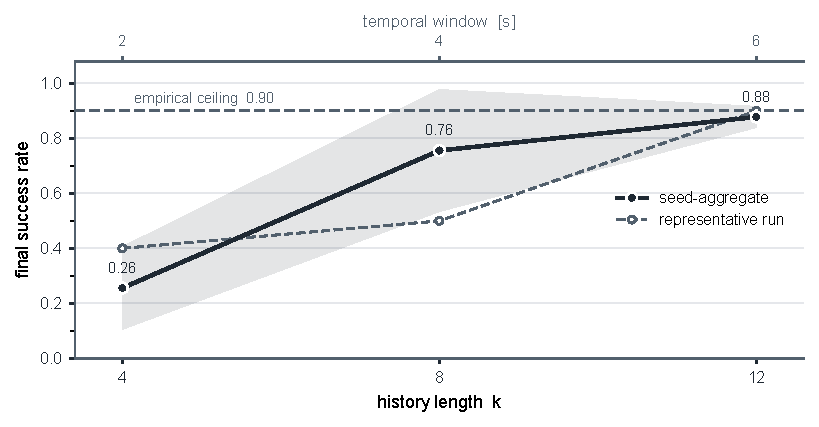
\includegraphics[width=138mm]{figures/fig_ch5_online_monotonic.pdf}
    \caption{临界工况下可部署单点 $s_0$ 的最终成功率与其跨重复训练离散度随观测历史长度 $k$ 的变化（终检评估；上轴为对应时序窗 $k\cdot\Delta t_{\mathrm{ctrl}}$，$\Delta t_{\mathrm{ctrl}}=0.5$ s）。深色为三次重复训练的聚合趋势（均值与种子带），浅色细线为三次训练各自的轨迹：两次沿 $k=4\to8\to12$ 未见回落，一次在高位持平后微降。判别力来自同一初始化下的跨历史长度对照，即 $k=8$ 时停在中途的那次训练在仅改变历史长度后被推到经验上界（$0.90$，灰色虚线）；离散度随 $k$ 的收窄与之一致，只作旁证。}
    \label{fig:ch5_online_monotonic}
\end{figure}

\begin{figure}[htbp]
    \centering
    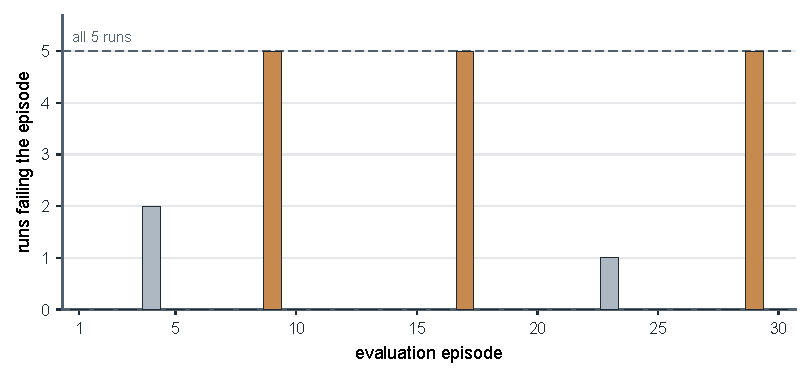
\includegraphics[width=138mm]{figures/fig_ch5_online_manifest_floor.pdf}
    \caption{评估集的经验上界。对评估集中的每个回合，统计有多少次充分训练的可部署训练未能完成它（越界或超时）。三个回合在全部训练中无一例外地失败（暖色），与历史长度和初始化无关，构成内在于评估集而非策略的上界 $27/30=0.900$；其余回合至多在个别训练中失败。可部署配置在 $k=12$ 恰好逼近这一上界。}
    \label{fig:ch5_online_manifest_floor}
\end{figure}

\subsection{对可部署策略设计的含义}\label{subsec:ch5_online_implications}

上述在线证据在本章的中心命题上给出一个明确的方向。临界工况下可部署性能的瓶颈，不在传感硬件的丰富程度，而在策略对既有单点观测的时序利用：把流场相位信息从时间维度上充分提取出来，比在空间上增设探针或在训练期为价值网络注入特权信息更直接地决定了可部署性能。这并不意味着空间感知没有作用：增设前向探针的 $s_1$ 确实闭合了差距，但空间探针在部署中不可得，其所提供的相位信息又可由对单点观测的充分时序利用替代；至于在训练期向价值网络注入特权信息，则在这一在线临界工况下并不闭合这一差距。因此，面向部署的改进路径不必指向更换或增设传感器，而可落在如何让策略更充分地利用单点观测的时序结构之上。

这一结论也划出了在线情形的一条参照水平。在临界工况下，仅用单点观测且仅作 $k=4$ 历史堆叠时，标准 SAC 的成功率均值约 $0.46$ 且在重复训练间剧烈分化，任务在在线交互下无法被可靠学得；而如前所示，同一工况下将历史窗延长到 $k=12$ 即可把成功率稳定抬升到空间参照的水平。这一时序救援依赖在线交互中可自由设定的观测历史长度，而离线情形只能复用既采数据既定的观测构成——本章离线各线所用数据均以 $k=4$ 采集。因此在线情形下靠延长时序窗闭合差距的途径，未必能直接迁移到离线；单点局部感知在离线、且更难工况下所能达到的水平，尚需在离线情形中单独考察。本章在后续考察失效边界时，即以这一在线参照为对照，界定单点局部感知在何种工况下仍支持可部署策略、又在何处触及不可逾越的边界。

\subsection{实施细节与可复现性}\label{subsec:ch5_online_impl}

亚临界工况的传感可行性考察在横流穿越任务上以标准 SAC 训练，三种传感配置各取三随机种子，每次训练 $60$ 万步，并行环境数固定为 $6$。该考察采用历史效率导向奖励，作为本章早期设定，其结论限于传感配置间的相对可学习性；其评估在专用于这一早期筛查的固定评估集上进行，周期评估与终检评估均每种子 $30$ 回合，区别于 \S\ref{subsec:ch5_eval} 定义的到达导向主评估集（主工况每种子 $100$ 回合）。所采用的历史效率导向奖励由一组在较短训练预算下进行的奖励权重筛选实验选定；该筛选只用于确定权重设定，其绝对成功率不作为性能基线，正式的可学习性与瓶颈分析均改用到达导向奖励。

临界工况下的传感配置比较（$s_0$、$s_1$、$s_2$）在横流穿越任务上以标准 SAC、到达导向奖励训练，三种配置各取三随机种子。瓶颈分析每次训练 $100$ 万步、并行环境数为 $6$，采用到达导向奖励与 $s_0$ 单点传感。特权信息消融在可部署基线上唯一启用价值网络的特权观测通道，策略网络保持单点观测；时序访问消融在同一基线上唯一改变观测历史长度（$k\in\{4,8,12\}$）。各项消融均只改变所述的单一因素，其余训练超参数与评估协议（\S\ref{subsec:ch5_eval}）保持一致。

本节表格与传感对比柱状图所报成功率为终检评估，学习曲线为周期评估，两者口径见 \S\ref{subsec:ch5_eval}；正文所称\emph{峰值}指某一配置周期评估序列的最大值，用于刻画该配置所能达到的水平。各项消融均为冻结其余条件的单变量受控对照，其结论按受控对照解读：传感比较与时序消融（$k\in\{4,8,12\}$）各取三随机种子，特权信息消融取两随机种子作配对复现。评估集经验上界由多次充分训练的可部署单点观测训练在同一评估集上的逐回合越界统计得到：当某一回合在全部训练中均失败时，将其计入内在于评估集的难达回合（图~\ref{fig:ch5_online_manifest_floor}）。

% 本节图较多：在进入 §5.6 前冲刷 §5.5 的浮动体，避免图浮入下一节正文（图密度所致）。
\clearpage
